\begin{minipage}{0.25\linewidth}	
	\subsection{Umrechnungen}
	\begin{tabular}{|l|l|}
		\hline
		kPa 				& $\frac{kN}{m^2}$ \\ \hline
		Pa					& $\frac{N}{m^2}$  \\ \hline
		kg					& 10 N				\\ \hline
		$\frac{kN}{m^3}$	& $10 \cdot \frac{g}{cm^3}$ \\ \hline
		$\frac{kN}{m^2}$	& $\frac{N}{mm}$	\\ \hline
		$\gamma_w=\frac{kN}{m^3}\cdot 10^{-6}$ & $\frac{kN}{cm^3}$ \\ \hline
		$M_E=\frac{kN}{m^2}\cdot 10^{-4}$ & $\frac{kN}{cm^2}$	\\ \hline
	\end{tabular}
\end{minipage}
\begin{minipage}{0.2\linewidth}
	
	\begin{tabular}{lll}
		
		tera	& T & 10$^{12}$ \\
		
		giga	& G & 10$^9$ \\
		
		mega	& M & 10$^6$ \\
		
		kilo	& k & 10$^3$ \\
		
		milli	& m & 10$^{-3}$ \\
		
		micro	& $\mu$ & 10$^{-6}$ \\
		
		nano	& n & 10$^{-9}$ \\
		
		pico	& p & 10${-12}$ \\
		
	\end{tabular}
	
\end{minipage}
\begin{minipage}{\linewidth}
	\begin{tabular}{l|p{0.2\linewidth}}
		\multicolumn{2}{c}{\textbf{Statistik} } \\ \hline
		
		Mittelwert							&	$ x_m = \frac{1}{n} \sum x_i $	\\
		
		Standardabweichung der Stichprobe	& 	$ s = \sqrt{ \frac{1}{n - 1} \sum (x_i - x_m)^2 } $ \\
		
		Charakteristischer Wert				&	$ s_{u,k} = \varphi_k' = x_m - \frac{s}{\sqrt{n} } \cdot c $
		$ \rightarrow$ c-Wert aus Tabelle; $ f = n - 1; p = 1 -\alpha$	\\ 
		
		Berechnungswert $ \varphi_d' $		&	$ \varphi_d' = arctan (\frac{tan \varphi_k'}{1.2}) $ \\ \hline
		
	\end{tabular}
\end{minipage}	
\begin{minipage}{\linewidth}
	
	\vspace{1cm}
	
\section{Flachfundationen}
	\subsection{Tragfähigkeit}
		\textbf{Vorgehen}
		\begin{enumerate}
			\item Einwirkende Kraft E$_d$ = F$_{z,tot}$
			\item Bruchspannung $\sigma_f $
			\item vorhandene Spannung $ \sigma_v = \frac{ F_{z,tot,d} }{ \bar{a} \cdot \bar{b} } $
			\item Nachweis $ E_d \leq R_d $
		\end{enumerate}
%	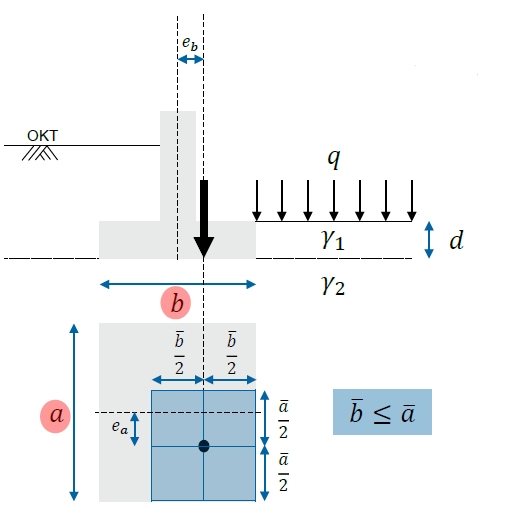
\includegraphics[width=0.7\linewidth]{images/Flachfun1allgTragfah.PNG}
\end{minipage}
\begin{minipage}{0.8\linewidth}
	
		\begin{tabular}{|l|l|p{0.25\linewidth}|}
			\hline
			Formel			&	Einheit		&	Bemerkung \\ \hline
			
			$ R_n
			= \bar{a} \cdot \bar{b} \cdot \sigma_f $ & [kN] & Bruchkraft; Achtung: Formel gilt für $ d/b \leq 2 $ \\ 
			$ \bar{a}
			= a - 2 \cdot e_a $ &	[m]		& reduzierter QS-Wert, wobei b $\leq$ a	\\
			$ e_a
			= \frac{M_y}{F_z} $ &	[m]		& Exzentrizität	\\
			$ \bar{b}
			= b - 2 \cdot e_b $ &	[m]		& reduzierter QS-Wert	\\
			$ e_b
			= \frac{M_x}{F_z} $ &	[m]		& Exzentrizität	\\
			$ \sigma_{f}
			= \gamma_2 \cdot \bar{b} \cdot N_b + ( \gamma_1 \cdot d + q ) \cdot N_d + c \cdot N_c $	& $ \left[\frac{kN}{m^3}\right] $ / [kPa]	& Bruchspannung,	c = Kohäsion \\		\hline
%			$ N_b
%			= N_{b0} \cdot \nu_b \cdot \iota_b \cdot \lambda_b \cdot \xi_b $
%			& $ \left[\frac{kN}{m^3}\right] $		&	\\
%			$ N_{b0}
%			= ( N_{d0} - 1 ) \cdot tan (\varphi) $ & [kN]	& undrainiert: $ N_{b0} = 0 $\\
%			$ N_d
%			= N_{d0} \cdot \nu_d \cdot \iota_d \cdot \lambda_d \cdot \xi_d $
%							& $ \left[\frac{kN}{m^3}\right] $		&	\\
%			$ N_{d0}
%			= e^{ \pi \cdot tan ( \varphi) } \cdot tan^2 ( 45° + \frac{\varphi}{2} ) $ & [kN]	& undrainiert: $ \varphi_u = 0 $;  $ N_{d0} = 1 $ \\
%						&		& drainier: $ \varphi ' > 0 $ 	\\
%			$ \nu_d
%			= 1 + \frac{\bar{b}}{\bar{a}} \cdot \sin(\varphi) $ &			&	\\
%			$ \iota_d
%			= ( 1 - tan(\delta))^m $	&		&	\\
%			$ \delta
%			= arctan \left( \frac{T}{F_z}\right) $		 & $\degree$		& 3 dimensionaler Winkel	\\
%			$ T
%			= \sqrt{F_x^2 + F_y^2} $ & $ \left[\frac{kN}{m^3}\right] $ &	Resultierende \\	
%			$ m
%			= m_a \cdot cos^2 (\omega) + m_b \cdot sin^2 (\omega) $ & &	\\
%			$ m_a
%			= \frac{2 + \frac{\bar{a}}{\bar{b}}}{1 + \frac{\bar{a}}{\bar{b}}} $ & & \\
%			$ m_b
%			= \frac{2 + \frac{\bar{b}}{\bar{a}}}{1 + \frac{\bar{b}}{\bar{a}}} $ & & \\	
%			$ \omega
%			= arctan \left[ \frac{F_y}{F_x} \right] $ &  & \\
%			$ \lambda_d
%			= 1 - 0.4 \cdot tan ( \beta ) $ &		&	\\ 
%			$ N_c
%			= N_{c0} \cdot \nu_c \cdot \iota_c \cdot \lambda_c \cdot \xi_c $
%			& $ \left[\frac{kN}{m^3}\right] $		&	\\
%			$ N_{c0}
%			= ( N_{d0} - 1) \cdot cot (\varphi) $ & [kN]	& undrainiert: $ N_{c0} = 2 + \pi $ \\ \hline
		\end{tabular}
	
\end{minipage}
\begin{minipage}{0.25\linewidth}
	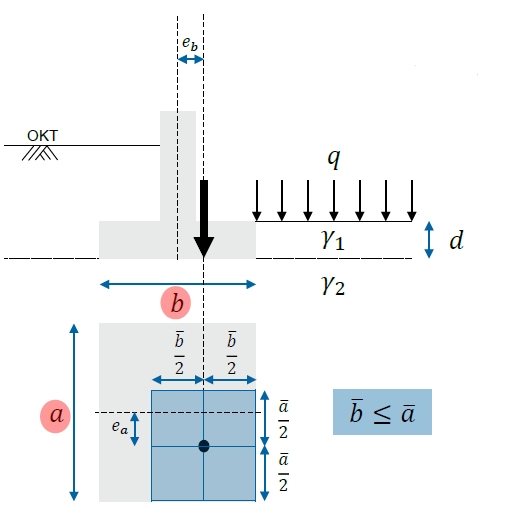
\includegraphics[width=\linewidth]{images/Flachfun1allgTragfah.PNG}
\end{minipage}


\begin{minipage}{0.85\linewidth}
	\begin{tabular}{l|l|p{0.2\linewidth}l}
		Bemerkung	& drainiert $ \varphi ' > 0 $	& undrainiert $ \varphi_u = 0 $ & \\ \hline
		
		Tragfähigkeitbeiwerte	& $ N_b
									= N_{b0} \cdot \nu_b \cdot \iota_b \cdot \lambda_b \cdot \xi_b $											& &	\\
								& $ N_d
								= N_{d0} \cdot \nu_d \cdot \iota_d \cdot \lambda_d \cdot \xi_d $	& & \\
								& $ N_c
								= N_{c0} \cdot \nu_c \cdot \iota_c \cdot \lambda_c \cdot \xi_c $ & & \\ \hline
								& $ N_{b0}
								= ( N_{d0} - 1 ) \cdot tan (\varphi) $	& $ N_{b0} = 0 $ & \\
								& $ N_{d0}
								= e^{ \pi \cdot tan ( \varphi) } \cdot tan^2 ( 45° + \frac{\varphi}{2} ) $ & $ N_{d0} = 1 $ & \\
								& $ N_{c0}
								= ( N_{d0} - 1) \cdot cot (\varphi) $ & $ N_{c0} = 2 + \pi $ & \\ \hline
		Formbeiwert				& $ \nu_b
								= 1 - 0.3 \cdot \frac{\bar{b}}{\bar{a}} $	& $ \nu_b = 1 $ & \\
								& $ \nu_d
								= 1 + \frac{\bar{b}}{\bar{a}} \cdot \sin(\varphi) $ & $ \nu_d = 1 $ & \\
								& $ \nu_c = \frac{\nu_d \cdot N_{d0} -1}{N_{d0} -1} $ & $ \nu_c = 1 + 0.2 \cdot \frac{\bar{b}}{\bar{a}} $ & \\ \hline
		Lastneigungsbeiwert $ \delta > 0 $		& $ \iota_b = (1 - tan ( \delta [\degree] ) ) ^{(m+1)} $	& & \\
								& $ \iota_d = (1 - tan ( \delta [\degree] ) ) ^m $	& $ \iota_d = 1 $  & \\
								& $ \iota_c = \frac{\iota_d \cdot N_{d0} -1}{N_{d0} -1} $ & $ \iota_c = \frac{1}{2} + \frac{1}{2} \cdot \sqrt{1 - \frac{T}{\bar{a} \cdot \bar{b} \cdot c_u}} $ $\rightarrow$ c$_u$ = s$_u$	& 				% 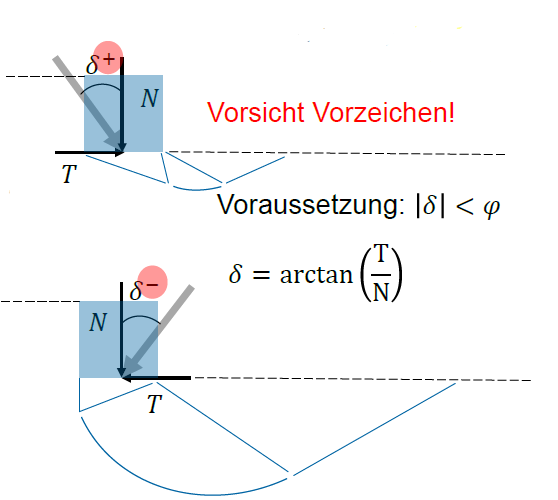
\includegraphics[width=0.2\linewidth]{images/Flachfun2Vorz.PNG} 
								\\
		Lastneigungsbeiwert $ \delta > 0 $ 	& $ \iota_b = cos ( \delta [\degree] ) \cdot (1 - 0.4 \cdot \delta [\degree]) ^{(0.64 + 0.028 \cdot \varphi [\degree])} $ & & \\
								& $ \iota_d = cos (\delta [\degree]) \cdot (1 - 0.0244 \cdot \delta [\degree]) ^{(0.03 + 0.04 \cdot \varphi [\degree])} $ & & \\
								& $ \iota_c = \frac{\iota_d \cdot N_{d0} -1}{N_{d0} -1} $ & & \\
								&&& \\
		3 dimensionaler Winkel	& $ \delta = arctan \left( \frac{T}{F_z}\right) $		 & 	& 	\\
		Resultierende			& $ T = \sqrt{F_x^2 + F_y^2} $ &  &	 \\
								& $ m = m_a \cdot cos^2 (\omega) + m_b \cdot sin^2 (\omega) $ & & \\
								& $ \omega = arctan \left[ \frac{F_y}{F_x} \right] $ &  & \\
								& $ m_a = \frac{2 + \frac{\bar{a}}{\bar{b}}}{1 + \frac{\bar{a}}{\bar{b}}} $ & & \\
								& $ m_b = \frac{2 + \frac{\bar{b}}{\bar{a}}}{1 + \frac{\bar{b}}{\bar{a}}} $ & & % 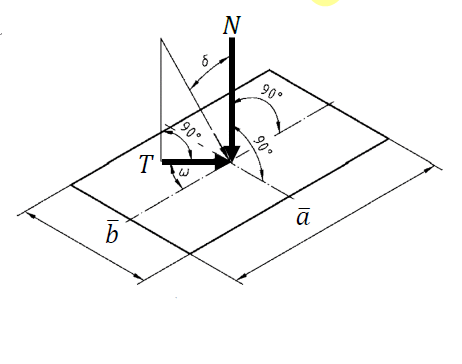
\includegraphics[width=0.2\linewidth]{images/Flachfun2Winkel.PNG} 
								\\ \hline
		Geländeneigungsbeiwert & $ \lambda_b = (1 - \frac{1}{2} \cdot tan (\beta [\degree] ) ) ^6 $ 	& & \\
								& $ \lambda_d = (1 - tan (\beta [\degree] ) ) ^{1.9} $	& $ \lambda_d = 1 $ & \\
								& $ \lambda_c = \frac{N_{d0} \cdot e ^{ (-0.0349 \cdot \beta [°] \cdot tan (\varphi [\degree] ) ) } -1 }{N_{d0} - 1} $	& $ \lambda_c = 1- 0.4 \cdot tan ( \beta [\degree] ) $ \\
								&	& $ \rightarrow $wenn $ \beta < \varphi $ & %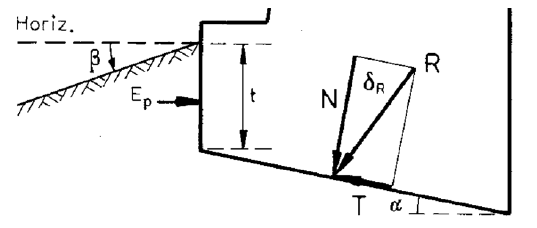
\includegraphics[width=0.2\linewidth]{images/Flachfun3Neig.PNG}
								\\ \hline 
		Sohlneigungsbeiwert		& $ \xi_b = e ^{(-0.045 \cdot \alpha [\degree] \cdot tan (\varphi [\degree]))} $	&	& \\
								& $ \xi_d = e ^{(-0.045 \cdot \alpha [\degree] \cdot tan (\varphi [\degree]))} $	& $ \xi_d = 1 $ & \\
								& $ \xi_c = e ^{(-0.045 \cdot \alpha [\degree] \cdot tan (\varphi [\degree]))} $ & $ \xi_c = 1 - 0.0068 \cdot \alpha [\degree] $ & %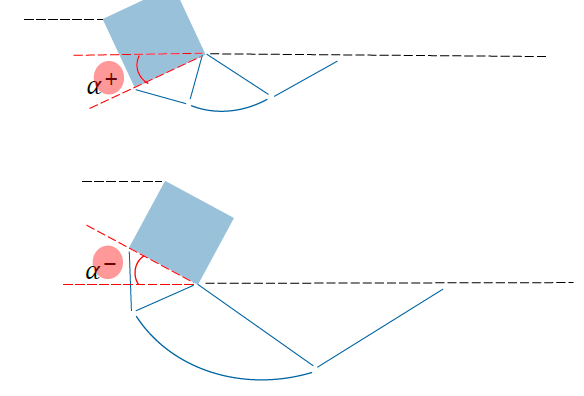
\includegraphics[width=0.2\linewidth]{images/Flachfun4Winkel.PNG} 
								\\ \hline			
		
	\end{tabular}
\end{minipage}
\begin{minipage}{0.2\linewidth}
	
	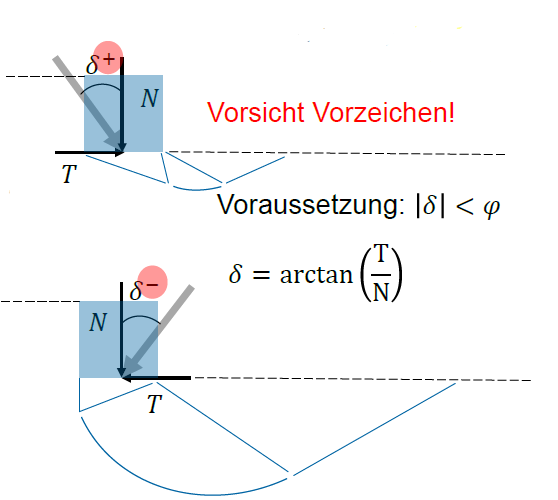
\includegraphics[width=\linewidth]{images/Flachfun2Vorz.PNG} \\
	
	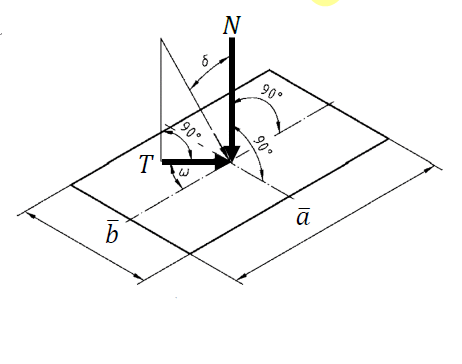
\includegraphics[width=\linewidth]{images/Flachfun2Winkel.PNG} \\
	
	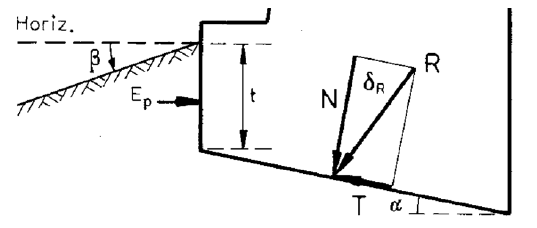
\includegraphics[width=\linewidth]{images/Flachfun3Neig.PNG} \\
	
	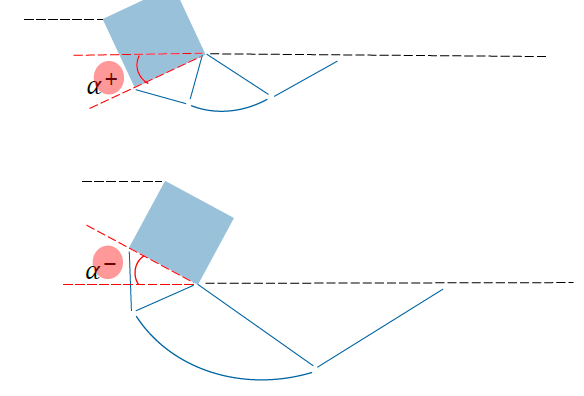
\includegraphics[width=\linewidth]{images/Flachfun4Winkel.PNG} \\
	
\end{minipage}


\textcolor{red}{Sicherheitsbeiwerte Geotech}



%	\subsection{Statistik}
	
%	\begin{minipage}{\linewidth}
%		\begin{tabular}{l|p{0.3\linewidth}}
%			 \hline
%			Mittelwert							&	$ x_m = \frac{1}{n} \sum x_i $	\\
%			
%			Standardabweichung der Stichprobe	& 	$ s = \sqrt{ \frac{1}{n - 1} \sum (x_i - x_m)^2 } $ \\
%				
%			Charakteristischer Wert				&	$ f = n - 1; p = 1 -\alpha$; c-Wert aus Tabelle $ \rightarrow s_{u,k} = \varphi_k' = x_m - \frac{s}{\sqrt{n} } \cdot c $	\\ 
%			
%			Berechnungswert $ \varphi_d' $		&	$ \varphi_d' = arctan (\frac{tan \varphi_k'}{1.2}) $ \\ \hline
%						
%		\end{tabular}
%	\end{minipage}	



%	\begin{minipage}{0.5\linewidth}
%		\subsection{Gebrauchstauglichkeit}
%			\subsubsection{Relative Steifigkeit}
%			$ k = \frac{1}{12} \frac{E}{M_E} \left( \frac{d}{l} \right)^3 $ \\
%		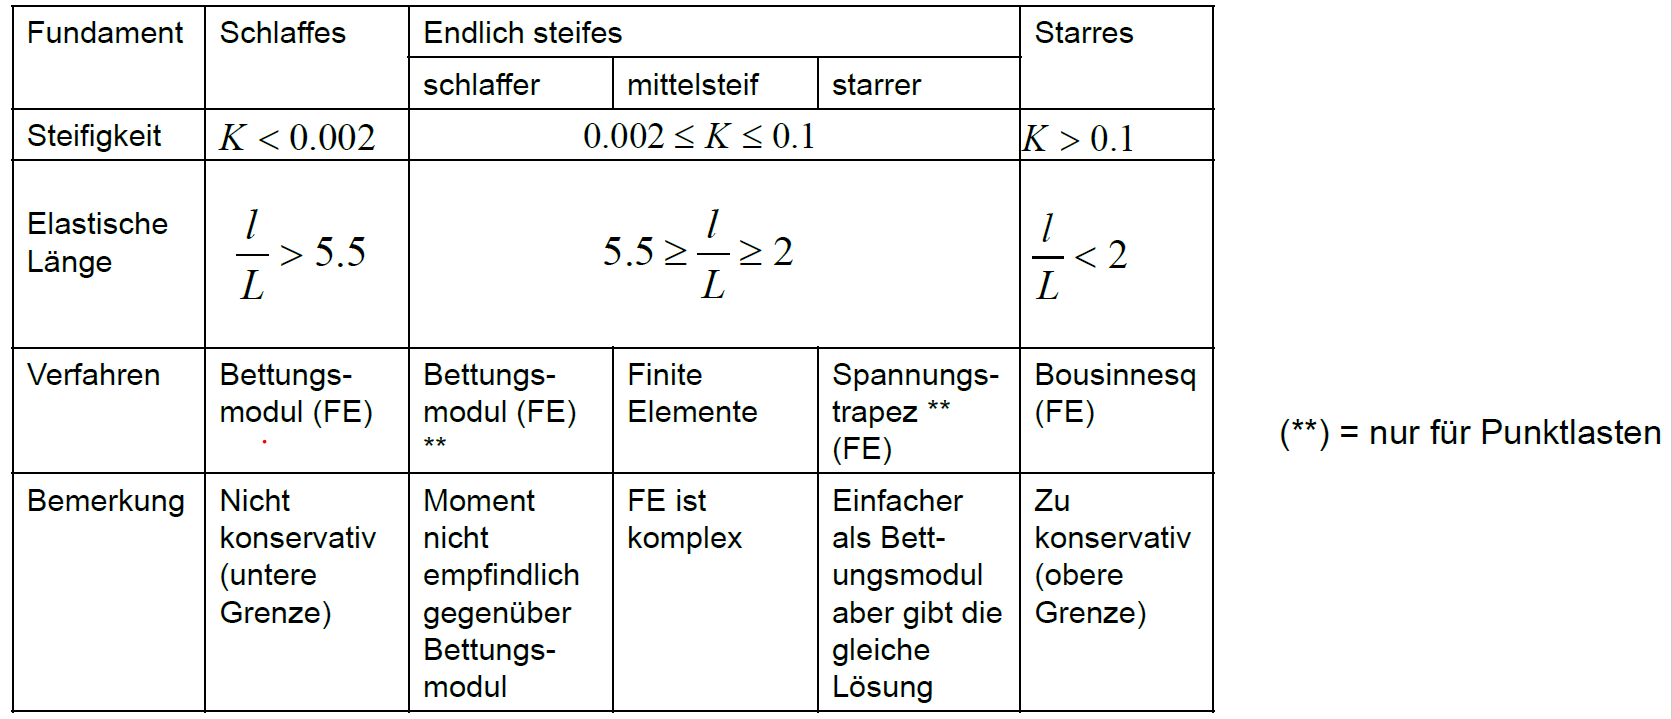
\includegraphics[width=\linewidth]{images/Flachfun5starrschlaff.PNG}
%	\end{minipage}
%	\begin{minipage}{0.3\linewidth}
%		\subsubsection{Spannungstrapezverfahren}
%		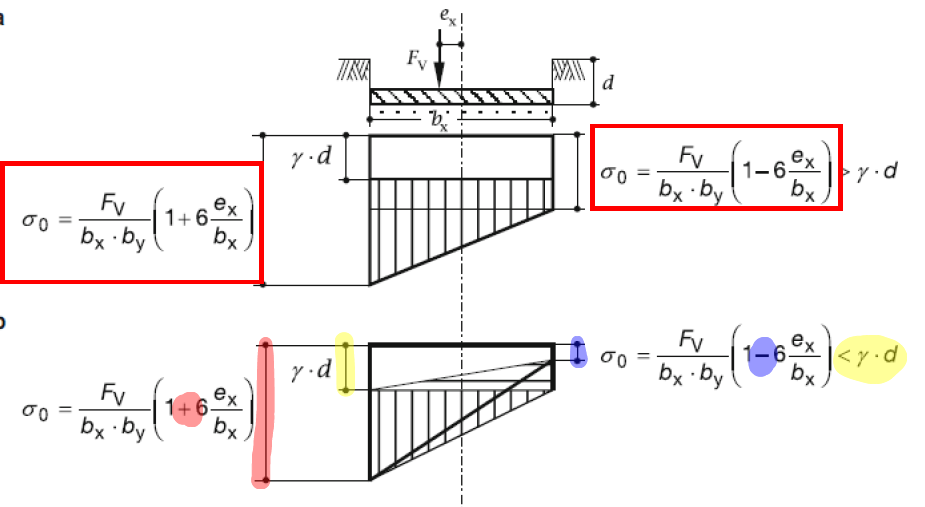
\includegraphics[width=\linewidth]{images/Flachfun6Sptrapez.PNG}
%	\end{minipage}


\clearpage


\begin{multicols}{2}


	\subsection{Bodenbauwerksinteraktion}
	Wann kommt welche Methode zum Einsatz?\\
	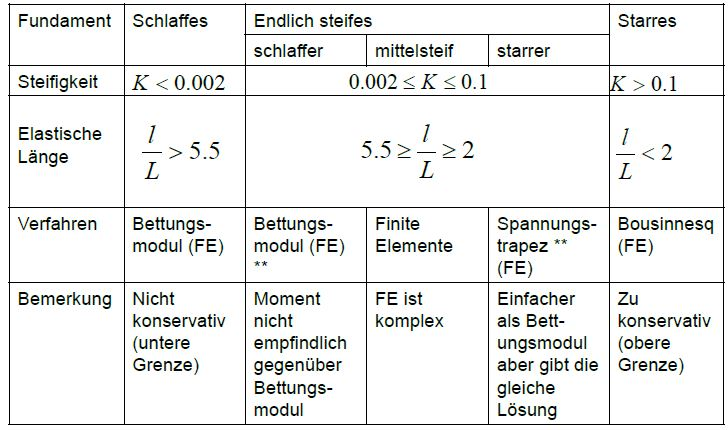
\includegraphics[width=1.0\linewidth]{images/Verfahren}\\
	\textbf{Vorgehen:}\\
	\begin{enumerate}
		\item Relative
		Steifigkeit bestimmen\\
		Allgemein: $K[-]=\frac{E\cdot I}{E_s\cdot l^3\cdot b}$\\
		Rechteckplatte bzw. -balken:
		$K[-]=\frac{E}{12\cdot E_s (=M_E)}\cdot (\frac{d}{l})^3$ \\
		Kreisplatten: $K[-]=\frac{E}{12\cdot E_s}\cdot(\frac{d}{D})^3$\\
		\begin{tiny}
			
			EI: Biegesteifigkeit des Gründungskörpers(Bauweks); E: E-Modul des Baustoffs(z.B. Beton); l: Länge des Bauwerks; b: Breite Bauwerk; d: Dicke des Balkens; D: Durchmesser der Kreisplatte; $E_s$: Steifemodul des Baugrunds
		\end{tiny}	
		\item 
		Verfahren auswählen:

		
	\end{enumerate}


	\subsubsection{Spannungstrapez}
	
	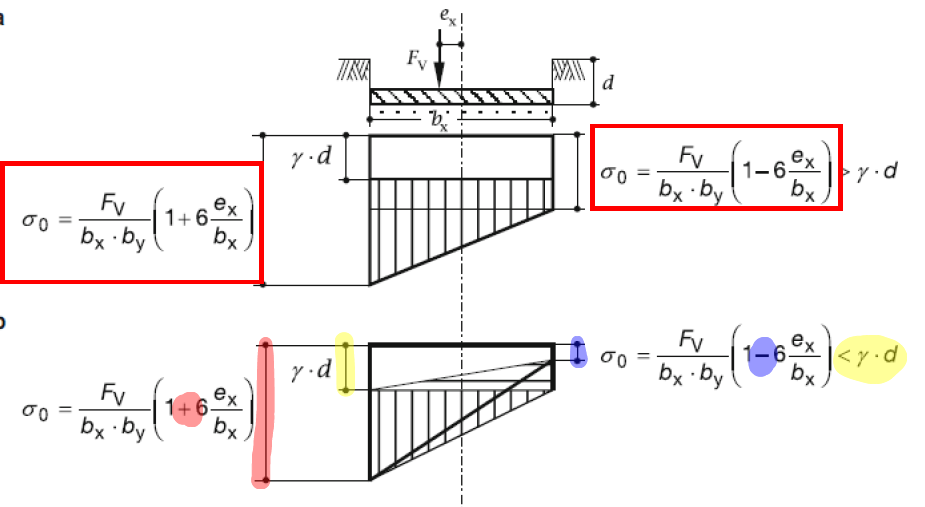
\includegraphics[width=\linewidth]{images/Flachfun6Sptrapez.PNG}
	
	\textbf{Vorgehen:}
	
	\begin{enumerate}
		\item 
		Resultierende im Kern?\\Koordinatensystem in Mitte setzen und e ausrechnen:\\
		$e=\frac{\sum p_i\cdot x_i}{\sum p_i}$\\
		$e\leq \frac{l}{6}$
		
		\item
		Sohlpressung berechnen(Anfang und Ende Balken)\\
		$q_{l/r}=\frac{Res}{b\cdot l}\pm\frac{6\cdot Res\cdot e}{l^2\cdot b} $
		
		\item 
		Querkräfte und Momente in den gewünschten Punkten berechnen:\\
		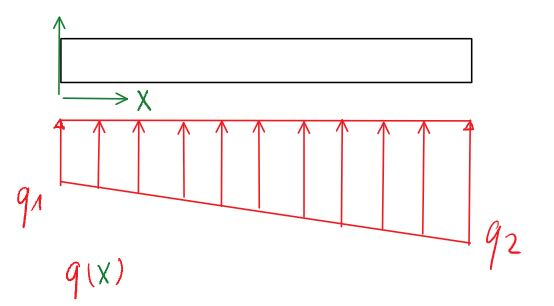
\includegraphics[width=0.7\linewidth]{images/Sohldruck}\\
		$q(x)=q_1+(\frac{q_2-q_1}{l})\cdot x$
		\item 
		Schnittkräfte bestimmen	
	\end{enumerate}
	
	\subsubsection{Bettungsmodulverfahren}
	Grundsatz: Biegelinie und Setzungsmulde sind gleich\\
	\textbf{Vorgehen:}
	\begin{enumerate}
		\item 
		Elastische Länge berechnen\\
		$L=(\frac{4\cdot E\cdot I}{K_s\cdot b})^\frac{1}{4}$ mit $K_s=\frac{M_E}{f\cdot b}$\\
		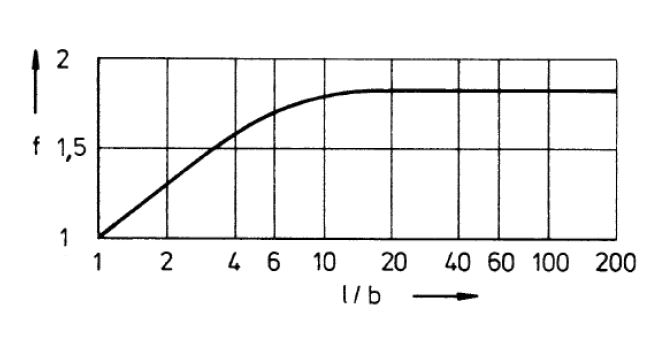
\includegraphics[width=1.0\linewidth]{images/f}
		\item 
		Wie verhält sich Balken\\
		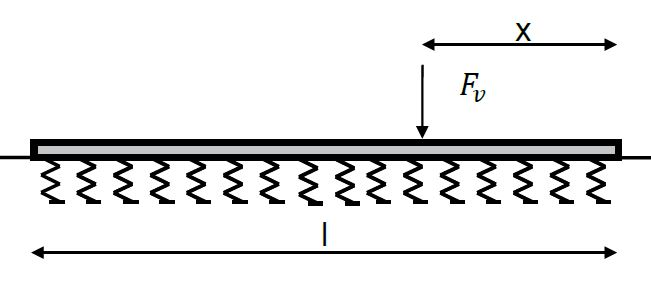
\includegraphics[width=1.0\linewidth]{images/Balken}
		\begin{itemize}
			
			\item 
			$\infty Balken : x > 2L$
			\item 
			$0.5 \infty  Balken: x < 2L$
			
		\end{itemize}
	\end{enumerate}
	\subsubsection{Bettungsmodulverfahren: Unendlich langer Balken}
	Wenn die Balkenlänge l grösser als 3L ist, kann man den Balken als unendlich lang ansehen und die Integrationskonstante $A_{3,4} = 0$ setzen.\\
	$A_1=A_2$\\
	L: elastische Länge\\
	l: effektive Länge\\
	$\xi=\frac{x}{L}$
	
	Elastisch Länge L:\\
	$L^4 = \frac{4EI}{b\cdot k_s}$
	<-->
	$L = \sqrt[4]{\frac{4EI}{b\cdot k_s}}$\\
	$M(\infty)=0=(A_1cos\xi + A_2sin\xi)\cdot e^{-\infty}+(A_3cos\xi + A_4sin\xi) \cdot e^\infty$\\
	$M(\xi)=\frac{F_v}{4}\cdot L\cdot e^{-\xi}\cdot(cos\xi - sin\xi)$\\
	$Q(\xi)=-\frac{F_v}{2}\cdot e^{-\xi}\cdot cos\xi$\\
	$s_z(\xi)=\frac{F_v}{2Lbk_s}\cdot e^{-\xi}\cdot(cos\xi+sin\xi)$ \\
	$ \sigma = k_s \cdot s $
	\subsubsection{Bettungsmodulverfahren: Halb unendlich langer Balken}
	$A_{1,3,4} = 0$ \\
	$A_2=-F_v\cdot L$\\
	L: elastische Länge\\
	l: effektive Länge\\
	
	Elastisch Länge L:\\
	$L^4 = \frac{4EI}{b\cdot k_s}$
	<-->
	$L = \sqrt[4]{\frac{4EI}{b\cdot k_s}}$\\
	$M(\infty)=0=(A_1cos\xi + A_2sin\xi)\cdot e^{-\infty}+(A_3cos\xi + A_4sin\xi) \cdot e^\infty$\\
	$M(\xi)=-F_v\cdot L\cdot sin\xi\cdot e^{-\xi} $\\
	$Q(\xi)=F_v\cdot (sin\xi - cos\xi) e^{-\xi}$\\
	$s_z(\xi)=\frac{2\cdot F_v}{Lbk_s}\cdot cos\xi\cdot e^{-\xi}$


	\subsubsection{Boussinesq}
	
	\begin{minipage}[t]{0.5\linewidth}
		$\rightarrow$ TR auf RAD!
		%	\vspace{\baselineskip} \\
		\subsection{Superposition}
		\begin{tabular}{ll}
			$\Delta \sigma_z=q \cdot J(a,b,z)$	& $\rightarrow a<b$ \\
			& $\rightarrow z=$Tiefe \\
			& $\rightarrow q=$Belastung $\left[\frac{kN}{m^2}\right]$ \\
			& $\rightarrow J=$Tab. s. 6.10f \\
			& $\rightarrow J=\frac{1}{2\cdot \pi} \cdot \left[arctan(\frac{a \cdot b}{R \cdot z}) + \frac{a \cdot b \cdot z}{R} \cdot  \left(\frac{1}{a^2 + z^2} + \frac{1}{b^2 + z^2}\right) \right]$ \\
			& $\rightarrow R^2=a^2 + b^2 + z^2$ \\	
		\end{tabular}
		
		% \textbf{vertikal Schnitt \& a,b-Feld} \\
		\vspace{\baselineskip}
	\end{minipage}
	\begin{minipage}[t]{0.3\linewidth}
		\vspace{2\baselineskip}
		\qquad 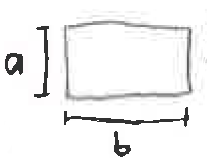
\includegraphics[width=0.7\linewidth]{images/SpimBoden1.PNG}
	\end{minipage}
	\begin{minipage}[t]{0.5\linewidth}
		\vspace{2\baselineskip}
		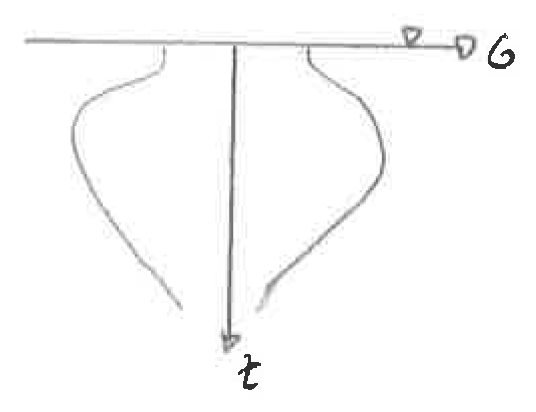
\includegraphics[width=0.4\linewidth]{images/SpimBoden2Verlauf.PNG}
	\end{minipage}
	
	
\end{multicols}

	
	\begin{minipage}{0.7\linewidth}
		\begin{tabular}{|l|l|l|l|l|l|l|l|}
			\hline
			Schicht	& $\Delta$ z	& z$_m$		& $\sigma`_zm$	& J$_{a/b/c}$	& $\Delta \sigma_{a/b/c}$ 	& $\varepsilon_{a/b/c}$ 	& $\Delta$s \\
			& [m]			& [m]		&  [kPa]		& 				& $\left[\frac{kN}{m^2}\right]$ &		& [m] \\ \hline
			
			&		& \multicolumn{2}{c|}{$\cdot (\gamma - \gamma_w)$} &		\multicolumn{2}{c|}{$\cdot q_{Auflast}$} & \multicolumn{2}{c|}{$\qquad \cdot \Delta z$} \\
			&	&	&	&	& \multicolumn{2}{c|}{$\frac{1}{E}$} & \\
			%next Line
			&	&	&	&	&\multicolumn{2}{c|}{ od. $\varepsilon=\frac{C_c}{1 + e_0} \cdot log \frac{\sigma`_z + \Delta \sigma}{\sigma`_z}$} & \\ \hline 	
		\end{tabular}
		\vspace{\baselineskip}
	\end{minipage}	
	\begin{minipage}{0.4\linewidth}
		\begin{tabular}{l|l|l|l}
			\hline
			z	&	$\frac{z}{R}$	&	$\frac{a}{R}$ (J)	&	J$_{def/int}$	\\ \hline
			& \qquad	t		&	J$_t$				&	\\
			&	x				&						& $J_t - (J_t - J_h) \cdot \frac{x - t}{h - t}$	\\
			& \qquad	h		&	J$_h$				&	\\
		\end{tabular}
		\vspace{\baselineskip} \\
	\end{minipage}
	
	
	
	\begin{minipage}{\linewidth}
		\begin{tabular}{|l|l|l|l|l|l|l|l|l|l|l|}
			\hline
			Schicht	& $\Delta$ z	& z$_m$		& $\sigma`_zm$	& J$_{a/b/c}$	& $\Delta \sigma_{a/b/c...w}$ 	& $\varepsilon_{a/b/c...w}$ 	& $\Delta s_w$ & $\Delta \sigma_E$ & $\varepsilon_E$ & $\Delta s_E$	\\
			%nxt Line
			& [m]			& [m]		&  [kPa]		& 				& $\left[\frac{kN}{m^2}\right]$ &		& [m] 	& $\left[\frac{kN}{m^2}\right]$ &		 & $\left[\frac{kN}{m^2}\right]$ \\ \hline
			\multicolumn{11}{|c|}{$\rightarrow$ $\Delta s = \Delta s_w + \Delta s_E$} \\
		\end{tabular}
		
		\vspace{\baselineskip}
	\end{minipage}
	
	
	\begin{minipage}{0.5\linewidth}
		$\rightarrow$ \textbf{linear}: \\
		$\Delta \sigma_w=$ Wiederbelastung $=z \cdot \gamma$ [kPa] \\
		$\Delta \sigma_E=$ Bodenpressung $=q - \sigma_w$ [kPa] \\
		q $=$ Zusatzbelastung \\
		$\varepsilon_w = \frac{\Delta \sigma_w}{M`_E}$ ; $\varepsilon_E = \frac{\Delta \sigma_E}{M_E}$ \\
		$\Delta s_w = \Delta z \cdot\varepsilon_w$ ; $\Delta s_E = \Delta z \cdot\varepsilon_E$\\
	\end{minipage}	
	\begin{minipage}{0.5\linewidth}
		$\rightarrow$ \textbf{logarithmisch} analog linear jedoch: \\
		$\varepsilon_w = \frac{c_s}{1 + e_0} \cdot log \frac{\sigma`_z + \Delta \sigma_w}{\sigma`_z}$ wobei $\sigma`_z =$ 100 kPa \\
		$\varepsilon_E = \frac{c_c}{1 + e_0} \cdot log \frac{\sigma`_z + \Delta \sigma_w + \Delta \sigma_E}{\sigma`_z + \Delta \sigma_w}$ wobei $\sigma`_z =$ 100 kPa \\
		$\Delta s_w= \varepsilon_w \cdot \Delta z$ ; $\Delta s_E= \varepsilon_E \cdot \Delta z$ \\
		\vspace{\baselineskip}
	\end{minipage}
	
%	\subsection{Differenzielle Setzungen}
%	\subsubsection{Nach Zilch}
%	
%	
%	\subsubsection{Setzungsberechnung starres Fundament}
	
	
	
%\end{multicols}


%\begin{minipage}{\linewidth}
%	\begin{tabular}{l|l|l}
%		Formel			&	Einheit	&	Bemerkung \\ \hline
%	\end{tabular}
%\end{minipage}